\documentclass[11pt]{article}

\usepackage{amsmath}
\usepackage[french, onelanguage]{algorithm2e}
\usepackage[french]{babel}
\usepackage{geometry}
\usepackage{glossaries}
\usepackage{graphicx}
\usepackage[hidelinks]{hyperref}
\usepackage[utf8]{inputenc}
\usepackage{listings}
\usepackage{lstautogobble}
\usepackage{tabularx}
\usepackage{tikz}
\usepackage{tocloft}
\usepackage{verbatim}
\usepackage{xcolor}

\makeglossaries

\newacronym{ansi}{ANSI}{American National Standard Institute}
\newacronym{ram}{RAM}{Random Access Memory}

\usetikzlibrary{calc, shapes.multipart, chains, arrows}

\geometry{
  a4paper,
  total={170mm,257mm},
  left=20mm,
  top=20mm,
}

\definecolor{RoyalBlue}{cmyk}{1, 0.50, 0, 0}

\lstset{language=C,
  keywordstyle=\color{RoyalBlue},
  basicstyle=\scriptsize\ttfamily,
  commentstyle=\ttfamily\itshape\color{darkgray},
  stringstyle=\ttfamily,
  breaklines=true,
  keepspaces=true,
  numbers=left,
  numbersep=5pt,
  showspaces=false,
  showstringspaces=false,
  showtabs=false,
  tabsize=4,
  autogobble=true
}

\title{Documentation Mini Projet Langage C}
\author{Caculli Giorgio, Jedrzej Tyranowski\\Haute École de Louvain en Hainaut (HELHa)}
\date{\today}

\begin{document}

\maketitle
\begin{abstract}
  Documentation pour le projet de Langage procédural sur les listes chaînées. Projet basé sur le concept
  d'un centre de formations.
\end{abstract}
%\small
\textbf{\textit{Mots-clés : }}liste, chaînée, c, noeud, centre, formation, tête

\newpage
\tableofcontents

\newpage
\section{Introduction}

\subsection{Le langage C}
La langage de programmation utilisé lors du développement et la mise en \oe{}uvre du programme est le
\texttt{ANSI-C}. Les différentes versions du langage disponibles lors du développement de ce programme sont:
\begin{itemize}
\item \textbf{ANSI-C} : La première vérsion standardisée par le \textbf{\acrlong{ansi}},
  abrégé en \textbf{\acrshort{ansi}} dans ce document, du langage \texttt{C} publiée en 1990.
\item \textbf{C-99} : Révision de la version \acrshort{ansi} pour permettre aux développeurs d'utiliser les
  commentaires \texttt{//}, les booléans grâce à la librairie \texttt{<stdbool.h>}, la déclaration des int
  directement dans la boucle \texttt{for}, et d'autres modérnisations de la syntaxe.
\item \textbf{C-11} : Mise à jour du langage \texttt{C} pour permettre le support des \texttt{thread} afin de pouvoir faire du multi-threading.
\item \textbf{C-17} : Révision de la version \textbf{C-11} qui n'ajoute aucune nouvelle fonctionnalité, mais
  corriges beaucoup bugs présents dans la version 11.
\end{itemize}
Dans les différentes applications que l'on a fait dans le cours de Langage procédural, la plupart des
interactions que l'on a eu avec le langage \texttt{C}, notammente le fait de devoir déclarer un \texttt{int}
avant une boucle \texttt{for}, ressemblaient fortement à l'\acrshort{ansi}-\texttt{C}. C'est pourquoi nous
avons choisi d'utiliser cette vérsion là.

\subsection{Fonctions générales utilisées}
Différentes fonctions ont été utilisée lors du développement de ce programme, ainsi que des MACRO pour
permettre au compilateur de reconnaître le système d'exploitation dans lequel le logiciel compilé tournera.
Voici une liste des fonctions clés utilisées:
\begin{itemize}
  
\item \texttt{fopen()} : Fonction qui sert à ouvrir un flux, plus précisement, un fichier.\\
  Exemple :
  \begin{lstlisting}
    /* Admettons que le fichier donnees.dat existe */
    #include <stdio.h>
    int main() {
      FILE *fichier_in = fopen( "donnees.dat", "r" );
      /* On ouvre le fichier donnees.dat en lecture */
      FILE *fichier_out = fopen( "resultats.txt", "w" );
      /* Si le fichier resultats.txt n'existe pas on le cree, s'il existe toute information presente est ecrasee, puis on y accede en ecrite */
      return 0;
    }
  \end{lstlisting}

\item \texttt{fclose()} : Fonction qui sert à fermer tout flux ouvert.\\
  Exemple :
  \begin{lstlisting}
    /* Admettons que le fichier donnees.dat existe */
    #include <stdio.h>
    int main() {
      FILE *fichier_in = fopen( "donnees.dat", "r" );
      /* On ouvre le fichier donnees.dat en lecture */
      FILE *fichier_out = fopen( "resultats.txt", "w" );
      /* Si le fichier resultats.txt n'existe pas on le cree, s'il existe toute information presente est ecrasee, puis on y accede en ecrite */
      fclose( fichier_out );
      fclose( fichier_in );
      /* On ferme les fichiers lorsqu'on doit plus travailler avec eux */
      return 0;
    }
  \end{lstlisting}

  
\item \texttt{printf()} : Fonction qui sert à afficher une châine de caractères dans la console.\\
  Exemple:
  \begin{lstlisting}
    #include <stdio.h>
    int main() {
      printf( "Hello World!\n" ); /* Affiche "Hello World!" dans la console */
      return 0;
    }
  \end{lstlisting}
  
\item \texttt{fprintf()} : Fonction qui sert à écrire une chaîne de caractères vers un flux spécifique.\\
  Exemple:
  \begin{lstlisting}
    #include <stdio.h>
    int main() {
      File *ficher_sortie = fopen( "fichier_sortie.txt", "w" );
      /* On cree et on ouvre un fichier nomme fichier_sortie.txt en ecriture */
      fprintf( ficher_sortie, "Hello World!\n" );
      /* Ecrit "Hello World!" dans le ficher fichier_sortie.txt mais pas dans la console */
      fprintf( stdout, "Hello World!\n" );
      /* Affiche "Hello World!" dans la console mais pas dans le fichier de sortie */
      return 0;
    }
  \end{lstlisting}

\item \texttt{scanf()} : Fonction qui sert à extrapoler une entrée du clavier et stocker les informations extrapolées dans les paramètres déclarés dans la fonction.\\
  Exemple:
  \begin{lstlisting}
    #include <stdio.h>
    int main() {
      char prenom[50];
      int age;
      printf( "Comment t'appels-tu ? " );
      scanf( "%s", prenom ); /* Admettons que l'utilisateur insere "Jedrzej" */
      printf( "Quel age as-tu %s ? ", prenom );
      scanf( "%d", &age ); /* Admettons que l'utilisateur insere "21" */
      printf( "Salut %s, je vois que tu as %d ans!\n", prenom, age );
      /* Affiche "Salut Jedrzej, je vois que tu as 21 ans!" dans la console */
      return 0;
    }
  \end{lstlisting}
  
\item \texttt{fscanf()} : Fonction qui sert à extrapoler des entrées à partir d'un flux spécifique en respectant une structure précise, et stocker les informations extrapolées dans des paramètres déclarés dans la fonction.\\
  Exemple:
  \begin{lstlisting}
    /* Contenu dans ficher_entree.txt */
    /* Jedrzej 21 */
    #include <stdio.h>
    int main() {
      char prenom[50];
      int age;
      FILE *ficher_in = fopen( "fichier_entree.txt", "r" );
      /* On ouvre un fichier nomme fichier_entree.txt en lecture */
      fscanf( fichier_in, "%s %d\n", prenom, &age );
      /* On lit le contenu de fichier_entree.txt */
      printf( "Salut %s, je vois que tu as %d ans\n", prenom, age );
      /* Affiche "Salut Jedrzej, je vois que tu as 21 ans!" dans la console */
      return 0;
    }
  \end{lstlisting}
  
\item \texttt{fgets()} : Fonction qui a le même principe que fscanf, mais garde les espaces.\\
  Exemble :
  \begin{lstlisting}
    /* Contenu dans fichier_entree.txt */
    /* Caculli Giorgio 23 */
    #include <stdio.h>
    int main() {
      char nom_prenom[15];
      int age;
      FILE *fichier_in = fopen( "fichier_entree.txt", "r" );
      fgets( nom_prenom, 16, fichier_in );
      /* Lit les 15 caracteres depuis le fichier de donnees fichier_entree.txt */
      fscanf( fichier_in, "%d", &age );
      /* Lit l'age depuis le fichier de donnees fichier_entree.txt */
      printf( "%s %d\n", nom_prenom, age );
      /* Affiche "Caculli Giorgio 23" dans la console */
      return 0;
    }
  \end{lstlisting}
  
\item \texttt{strcpy()} : Fonction qui sert à copier une chaîne de caractères vers une autres chaîne de caractères.\\
  Exemple :
  \begin{lstlisting}
    #include <stdio.h>
    #include <string.h>
    int main() {
      char prenom[10];
      char source[10] = "Giorgio";
      strcpy( prenom, source );
      printf( "%s\n", prenom ); /* Affiche "Giorgio" dans la console */
      return 0;
    }
  \end{lstlisting}
  
\item \texttt{sizeof()} : Fonction qui renvoie la quantité de mémoire (en bytes) qu'une entité va occuper dans la \acrlong{ram}, ou mémoire vive en français, abrégé en \acrshort{ram} dans ce document.\\
  Exemple :
  \begin{lstlisting}
    #include <stdio.h>
    int main() {
      printf( "Taille de char: %lu\n", sizeof( char ) );
      /* Affiche 1 dans la console */
      printf( "Taille de int: %lu\n", sizeof( int ) );
      /* Affiche 4 dans la console */
      printf( "Taille de long: %lu\n", sizeof( long ) );
      /* Affiche 8 dans la console */
      printf( "Taille de int[4]: %lu\n", sizeof( int[4] ) );
      /* Affiche 16 dans la console, soit 4*4=16 */
      return 0;
    }
  \end{lstlisting}

\item \texttt{memcpy()} : Fonction qui copiés n octets depuis une zone mémoire vers une autre zone mémoire.\\
  Exemple :
  \begin{lstlisting}
    #include <stdio.h>
    #include <string.h>
    int main() {
      int src[] = {1, 2, 3};
      size_t n = sizeof(src) / sizeof(src[0])
      /* En sachant que la taille d'un int = 4 bytes, et qu'il y a 3 int dans src, on obtient 4 * 3 = 12 bytes utilises. On divise la taille totale du vecteur, soit 12, par la taille du premier element du vecteur, soit 4, donc 12 / 4 = 3 elements dans le vecteur */
      int dest[n]; /* On initialiser le vecteur dest avec la meme taille de src, ici 3 */
      memcpy( dest, src, sizeof(dest) ); /* On copie les informations de src vers dest */
      int i;
      for( i = 0; i < n; i++ ) {
        /* On parcourt tous les elements dans dest, du premier (indice 0) jusqu'au troisieme (indide 2) */
        printf( "%d ", dest[i] ); /* Affiche 1 2 3 dans la console */
      }
      return 0;
    }
  \end{lstlisting}
  
\item \texttt{getchar()} : Fonction qui sert à lire un caractère depuis un flux.\\
  Exemple:
  \begin{lstlisting}
    #include <stdio.h>
    int main() {
      char lettre;
      printf( "Inserez une lettre: " ); /* Admettons que l'utilisateur insere "a" */
      char c = getchar();
      printf( "Lettre inseree : %c\n", c );
      /* Affiche "a" dans la console */
    }
  \end{lstlisting}

\item \texttt{system()} : Fonction qui permet de lancer l'execution d'une commande sur le système d'exploitation hôte.\\
  Exemple:
  \begin{lstlisting}
    #include <stdlib.h>
    int main() {
      char *commande = "dir";
      system( commande );
      /* Execute la commande "dir", fonction qui sert a afficher ce qui est present dans le repertoire */
      return 0;
    }
  \end{lstlisting}

\item \texttt{calloc()} : Fonction qui permet de faire de l'allocation dynamique de mémoire.\\
  Exemple:
  \begin{lstlisting}
    #include <stdio.h>
    #include <stdlib.h>
    int main() {
      int *pointer;
      int i, n;
      printf( "Nombres d'elements a ajouter: " );
      scanf( "%d", &n ); /* Admettons que l'utilisateur insere 3 */
      pointer = ( int * ) calloc( n, sizeof( int ) );
      for( i = 0; i < n; i++ )
      {
        printf( "Entrez le numero N.%d ", i + 1 );
        scanf( "%d", &pointer[i] ); /* Admettons que l'utilisateur insere 1 2 et 3 */
      }
      for( i = 0; i < n; i++ )
      {
        printf( "%d ", pointer[i] );
        /* Affiche 1 2 3 dans la console */
      }
      return 0;
    }
  \end{lstlisting}
  
\end{itemize}

\subsubsection{Qu'est-ce l'allocation dynamique de mémoire?}
Une allocation dynamique de mémoire est le processus d'alluer de la mémoire lors de l'exécution d'un programme. Il existe quatre fonctions en \texttt{C} qui peuvent être utilisée pour allouer et libérer de la mémoire: \texttt{calloc()}, \texttt{free()}, \texttt{realloc()} et \texttt{malloc()}. Ces fonctions sont accéssible lors de l'introduction du header \texttt{<stdlib.h>} dans le code.

\subsubsection{Qu'est-ce \texttt{calloc()} ?}
\texttt{calloc()} est une fonction qui renvoie un pointeur vers un espace mémoire suffisamment libre pour stocker un tableau au nombre d'objets indéterminé et à la taille spécifiée. Si c'est pas le cas, la fonction renverra \texttt{NULL}. Le stockage est initialisé à zéro.

\subsubsection{Qu'est-ce \texttt{malloc()} ?}
\texttt{malloc()} est une fonction qui renvoie un pointeur vers un espace mémoire non initialisé. Si l'allocation n'est pas possible, la fonction renverra \texttt{NULL}. Si l'espace affecté par l'allocation est saturé, les résultats ne seront pas définis.

\subsubsection{Différences entre \texttt{calloc()} et \texttt{malloc()}}
\begin{center}
  \begin{tabularx}{\textwidth}{| >{\centering\arraybackslash}X | >{\centering\arraybackslash}X |}
    \hline
    \textbf{\texttt{malloc()}} & \textbf{\texttt{calloc()}} \\ 
    \hline
    \texttt{void * malloc( size\_t n );} & \texttt{void * calloc( size\_t n, size\_t size );} \\
    \hline
    \texttt{malloc()} prend un argument (le nombre d'octets)  & \texttt{calloc()} prend deux arguments (le nombre de blocs et la taille de chaque bloc)  \\
    \hline
    \texttt{malloc()} est plus rapide que \texttt{calloc()} & \texttt{calloc()} prends plus de temps que \texttt{malloc()} car la mémoire doit être initialisée à zéro \\
    \hline
  \end{tabularx}
\end{center}

\newpage
\section{Listes chaînées}
Voici une représentation d'une liste chaînée: 
\begin{tikzpicture}[list/.style={
      rectangle split,
      rectangle split parts=2,
      draw,
      rectangle split horizontal
    },
    >=stealth,
    start chain]

  \node[list,on chain] (A) {12};
  \node[list,on chain] (B) {99};
  \node[list,on chain] (C) {37};
  \node[on chain,draw,inner sep=6pt] (D) {};
  \draw (D.north east) -- (D.south west);
  \draw (D.north west) -- (D.south east);
  \draw[*->] let \p1 = (A.two), \p2 = (A.center) in (\x1,\y2) -- (B);
  \draw[*->] let \p1 = (B.two), \p2 = (B.center) in (\x1,\y2) -- (C);
  \draw[*->] let \p1 = (C.two), \p2 = (C.center) in (\x1,\y2) -- (D);
\end{tikzpicture}

\subsection{Qu'est-ce une liste chaînée?}
Une liste chaînée est une séquence de structures de données, qui sont liée par des n\oe{}uds.
Chaque n\oe{}ud contient une connexion vers un autre n\oe{}ud.\\
Voici à quoi ressemble une structure pour une liste chaînée linéaire en \texttt{C}:
\begin{lstlisting}
  typedef struct noeud
  {
    int donnee;         /* L'information que l'on souhaite stocker dans le noeud */
    struct noeud *suivant; /* Le lien vers le prochain noeud */
  } noeud;
  noeud *tete = NULL;   /* Le point de demarrage d'une liste chainee */
\end{lstlisting}

Contrairement à un vecteur, qui lui ressemblerait à ça:
\begin{lstlisting}
  int donnee[10];
\end{lstlisting}

Les deux vont très bien stocker des \texttt{int} que l'on a nommé \texttt{donnee}, cependant, un vecteur possède une taille fixe, il ne saura stocker que 10 éléments maximum dans notre cas. Tandis que dans le cas d'une liste chaînée, tant qu'il y a de l'espace en mémoire, il saura stocker un nombre indéfini de n\oe{}uds, et par conséquent, un nombre indéfini de \texttt{int donnee}.

\subsection{Création d'un nouveau n\oe{}ud}
Afin de pouvoir créer un n\oe{}ud que l'on stockera dans notre liste chaînée, il faudra d'abord lui alluoer une taille dans la mémoire. Toujours en se basant par le bout de code vu précédemment, et le bout de code vu dans le chapitre précédent sur l'allocation de mémoire, on obtiendrait le code suivant:
\begin{lstlisting}
  noeud *creer_noeud( int data )
  {
    noeud *temporaire = ( noeud * ) calloc( 1, sizeof( noeud ) );
    /* On cree un noeud temporaire ou l'on stockera les informations que l'on souhaite */
    temporaire->data = data; /* La donnee que l'on souhaite stocker */
    temporaire->suivant = NULL; /* Lien vers le prochain noeud s'il existe */
    return tmp; /* On retourne le noeud qui sera stocke dans la liste chainee */
  }
  noeud *treinte_sept = creer_noeud( 37 );
  free( treinte_sept );
\end{lstlisting}
Le résultat obtenu serait un n\oe{}ud du style:
\begin{tikzpicture}[list/.style={
      rectangle split,
      rectangle split parts=2,
      draw,
      rectangle split horizontal
    },
    >=stealth,
    start chain]
  \node[list,on chain] (C) {37};
\end{tikzpicture}

Le langage \texttt{C} ne fait pas de \texttt{Garbage Collection}, ce qui revient à dire que toute manipulation de mémoire doit être manipulée manuellement. Donc, lorsqu'on a besoin de libérer de la mémoire de données que l'on peut écraser, on utilise la fonction \texttt{free()}.\\
Dans ce cas-ci, le n\oe{}ud est créé mais il n'est pas encore stocké dans la liste chaînée.
On verra dans la section suivant comment on peut stocker ce nouveau noeud dans la liste chaînée.

\subsection{Insertion d'un n\oe{}ud dans une liste chaînée}
À l'état actuel des choses, on peut supposer que la liste chaînée soit vide: 
\begin{tikzpicture}[list/.style={
      rectangle split,
      rectangle split parts=2,
      draw,
      rectangle split horizontal
    },
    >=stealth,
    start chain]
  \node[on chain,draw,inner sep=6pt] (D) {};
  \draw (D.north east) -- (D.south west);
  \draw (D.north west) -- (D.south east);
\end{tikzpicture}\\
Une procédure d'ajout dans une liste chaînée pourrait être la suivante:
\begin{enumerate}
\item On initialise le noeud temporaire que l'on ajoutera à la base de données.
\item On associe \texttt{data} au pointeur \texttt{data} présent dans la structure \texttt{noeud}.
\item On initialise le prochain n\oe{}ud de la liste \texttt{*suivant} à NULL.
\item Si la tête \texttt{*tete} de la liste est \texttt{NULL}, alors la tête devient le nouveau n\oe{}ud. On arrête la fonction d'ajout là.
\item Sinon, on fait une copie de la tête dans le n\oe{}ud \texttt{*suivant} que l'on avait initialisé à \texttt{NULL}.
\item On déclare la tête comme étant le n\oe{}ud temporaire que l'on a initialisé.
\end{enumerate}
Dans une fonction, cette procédure ressemblerait à ça:
\begin{lstlisting}
  int ajouter_noeud( noeud *tete, int data )
  {
    noeud *temporaire = creer_noeud( data );
    /* On cree le noeud temporaire qui stocke la donnee */
    if( tete == NULL )
    {
      tete = temporaire;
      /* On le stocke directement temporaire a la place de tete si tete est NULL */
      return 1;
    }
    temporaire->suivant = tete;
    /* On fait une copie de tete (le noeud stocke precedemment) dans le suivant du noeud temporaire (au lieu de le laisser a NULL) */
    tete = temporaire;
    /* On fait devenir le noeud temporaire la nouvelle tete */
    return 1;
  }
  noeud *tete = NULL;
  ajouter_noeud( tete, 37 );
\end{lstlisting}
Si la fonction a réussi, la liste chaînée ressemblera à ça: 
\begin{tikzpicture}[list/.style={
      rectangle split,
      rectangle split parts=2,
      draw,
      rectangle split horizontal
    },
    >=stealth,
    start chain]
  \node[list,on chain] (C) {37};
  \node[on chain,draw,inner sep=6pt] (D) {};
  \draw (D.north east) -- (D.south west);
  \draw (D.north west) -- (D.south east);
  \draw[*->] let \p1 = (C.two), \p2 = (C.center) in (\x1,\y2) -- (D);
\end{tikzpicture}

Admettons que l'on souhaite ajouter une autre donnée à notre liste chaînée, on refait appel à la fonction:
\begin{lstlisting}[firstnumber=16]
  ajouter_noeud( tete, 99 );
\end{lstlisting}

Si la fonction a réussi, la liste chaînée ressemblera à ça:
\begin{tikzpicture}[list/.style={
      rectangle split,
      rectangle split parts=2,
      draw,
      rectangle split horizontal
    },
    >=stealth,
    start chain]
  \node[list,on chain] (B) {99};
  \node[list,on chain] (C) {37};
  \node[on chain,draw,inner sep=6pt] (D) {};
  \draw (D.north east) -- (D.south west);
  \draw (D.north west) -- (D.south east);
  \draw[*->] let \p1 = (B.two), \p2 = (B.center) in (\x1,\y2) -- (C);
  \draw[*->] let \p1 = (C.two), \p2 = (C.center) in (\x1,\y2) -- (D);
\end{tikzpicture}

\subsection{Suppression d'un n\oe{}ud d'une liste chaînée}

Pour que l'on puisse supprimer un n\oe{}ud, il faudra d'abord passer par différentes étapes de vérification:
\begin{enumerate}
\item On vérife que la tête de la liste \texttt{*tete} ne soit pas \texttt{NULL}, si oui, on arrête la fonction.
\item On vérifie si le premier élément de la liste correspond à la donnée \texttt{data} de la liste que l'on souhaite supprimer.
\item Si oui:
  \begin{enumerate}
  \item On crée un n\oe{}ud temporaire qui stockera la donnée suivante dans la liste.
  \item On libére l'espace mémoire occupé par head avec la fonction \texttt{free(tete)}.
  \item On attribue à \texttt{tete} le n\oe{}ud temporaire que l'on avait créé.
  \item On arrête la fonction.
  \end{enumerate}
\item Sinon, on parcourt l'entièreté de la liste jusqu'au moment où l'on trouve la formation qui a le même \texttt{donnee} que la \texttt{donnee} en paramètre.
\item Si on le trouve, on pivote l'élément qui suit vers l'élément que l'on vient de supprimer.
\item On arrête la fonction, si réussite, on obtient 1, si pas, on obtient 0.
\end{enumerate}

Cette procédure pourrait être écrite de la manière suivante:
\begin{lstlisting}
  int supprimer_noeud( noeud *tete, int data )
  {
    if( tete == NULL )
    {
      return 0;
    }
    noeud *temporaire = NULL;
    if( tete->data == data )
    {
      temporaire = tete->suivant;
      free( tete );
      tete = temporaire;
      return 1;
    }
    while( tete != NULL )
    {
      if( tete->suivant->data == data )
      {
        temporaire = tete->suivant;
        tete->suivant = tete->suivant->suivant;
        free( temporaire );
        return 1;
      }
      tete = tete->suivant;
    }
    return 0;
  }
  noeud *tete = NULL;
  ajouter_noeud( tete, 37 );
  ajouter_noeud( tete, 99 );
  ajouter_noeud( tete, 42 );
  ajouter_noeud( tete, 12 );
  ajouter_noeud( tete, 10 );
  supprimer_noeud( tete, 10 );
  supprimer_noeud( tete, 42 );
\end{lstlisting}

Analysons ce que le code fait:
\begin{enumerate}
  \setcounter{enumi}{26}
\item On crée la tête à NULL
\item On ajoute dans la liste chaînée la variable 37 qui sera stockée dans un n\oe{}ud.
\item On ajoute dans la liste chaînée la variable 99 qui sera stockée dans un n\oe{}ud.
\item On ajoute dans la liste chaînée la variable 42 qui sera stockée dans un n\oe{}ud.
\item On ajoute dans la liste chaînée la variable 12 qui sera stockée dans un n\oe{}ud.
\item On ajoute dans la liste chaînée la variable 10 qui sera stockée dans un n\oe{}ud.\\
  À l'état actuel des choses, la liste ressemble à ça:\\\\
  \begin{tikzpicture}[list/.style={
        rectangle split,
        rectangle split parts=2,
        draw,
        rectangle split horizontal
      },
      >=stealth,
      start chain]

    \node[list,on chain] (A) {10};
    \node[list,on chain] (B) {12};
    \node[list,on chain] (C) {42};
    \node[list,on chain] (D) {99};
    \node[list,on chain] (E) {37};
    \node[on chain,draw,inner sep=6pt] (F) {};
    \draw (F.north east) -- (F.south west);
    \draw (F.north west) -- (F.south east);
    \draw[*->] let \p1 = (A.two), \p2 = (A.center) in (\x1,\y2) -- (B);
    \draw[*->] let \p1 = (B.two), \p2 = (B.center) in (\x1,\y2) -- (C);
    \draw[*->] let \p1 = (C.two), \p2 = (C.center) in (\x1,\y2) -- (D);
    \draw[*->] let \p1 = (D.two), \p2 = (D.center) in (\x1,\y2) -- (E);
    \draw[*->] let \p1 = (E.two), \p2 = (E.center) in (\x1,\y2) -- (F);
  \end{tikzpicture}
\item On supprime le noeud avec la valeur 10.
\item On supprime le noeud avec la valeur 42.\\
  Au final la liste ressemblera à ça:\\\\
  \begin{tikzpicture}[list/.style={
        rectangle split,
        rectangle split parts=2,
        draw,
        rectangle split horizontal
      },
      >=stealth,
      start chain]

    \node[list,on chain] (A) {12};
    \node[list,on chain] (B) {99};
    \node[list,on chain] (C) {37};
    \node[on chain,draw,inner sep=6pt] (D) {};
    \draw (D.north east) -- (D.south west);
    \draw (D.north west) -- (D.south east);
    \draw[*->] let \p1 = (A.two), \p2 = (A.center) in (\x1,\y2) -- (B);
    \draw[*->] let \p1 = (B.two), \p2 = (B.center) in (\x1,\y2) -- (C);
    \draw[*->] let \p1 = (C.two), \p2 = (C.center) in (\x1,\y2) -- (D);
  \end{tikzpicture}
\end{enumerate}

Voici comment la suppression interagit avec la liste chaînée et le nombre 10:
\begin{enumerate}
\item Est-ce que le liste est vide? (\texttt{tete == NULL} ?)
  \begin{enumerate}
  \item Non car on a des noeuds dans notre liste, on continue dans la fonction.
  \end{enumerate}
\item Est-ce que la donnée \texttt{data} équivaut à la donnée \texttt{tete->donnee} ?
  \begin{enumerate}
    \item Oui car \texttt{tete->donnee = 10} et \texttt{data = 10}.
  \end{enumerate}
\item On fait un backup de \texttt{tete->suivant} dans un n\oe{}ud temporaire.
\item On libére le n\oe{}ud \texttt{tete}.
\item On attribue à \texttt{tete} le n\oe{}ud temporaire.\\
A ce stade de la modification, la liste ressemble à ça:\\\\
  \begin{tikzpicture}[list/.style={
        rectangle split,
        rectangle split parts=2,
        draw,
        rectangle split horizontal
      },
      >=stealth,
      start chain]
    \node[list,on chain] (B) {12};
    \node[list,on chain] (C) {42};
    \node[list,on chain] (D) {99};
    \node[list,on chain] (E) {37};
    \node[on chain,draw,inner sep=6pt] (F) {};
    \draw (F.north east) -- (F.south west);
    \draw (F.north west) -- (F.south east);
    \draw[*->] let \p1 = (B.two), \p2 = (B.center) in (\x1,\y2) -- (C);
    \draw[*->] let \p1 = (C.two), \p2 = (C.center) in (\x1,\y2) -- (D);
    \draw[*->] let \p1 = (D.two), \p2 = (D.center) in (\x1,\y2) -- (E);
    \draw[*->] let \p1 = (E.two), \p2 = (E.center) in (\x1,\y2) -- (F);
  \end{tikzpicture}
\end{enumerate}

Voici comment la suppression interagit avec la liste chaînée et le nombre 42:
\begin{enumerate}
\item Est-ce que le liste est vide? (\texttt{tete == NULL} ?)
  \begin{enumerate}
  \item Non car on a des noeuds dans notre liste, on continue dans la fonction.
  \end{enumerate}
\item Est-ce que la donnée \texttt{data} équivaut à la donnée \texttt{tete->donnee} ?
  \begin{enumerate}
    \item Non car \texttt{tete->donnee = 12} et \texttt{data = 42}.
  \end{enumerate}
\item On commence à parcourir toute la liste tant que \texttt{tete != NULL}.
\item On vérifie si \texttt{tete->suivant->donnee == data}
  \begin{enumerate}
  \item Si c'est pas le cas, on continue à parcourir la liste.
  \end{enumerate}
\item Si c'est le cas, on fait un backup du suivant du suivant dans un n\oe{}ud temporaire.
\item On libère \texttt{tete->suivant}.
\item On attribue à \texttt{tete->suivant} le n\oe{}ud \texttt{tete->suivant->suivant} (on pivote la liste vers la gauche et on libère l'espace mémoire qui était occupée par le 42).\\
A ce stade de la modification, la liste ressemble à ça:\\\\
  \begin{tikzpicture}[list/.style={
        rectangle split,
        rectangle split parts=2,
        draw,
        rectangle split horizontal
      },
      >=stealth,
      start chain]
    \node[list,on chain] (A) {12};
    \node[list,on chain] (B) {99};
    \node[list,on chain] (C) {37};
    \node[on chain,draw,inner sep=6pt] (D) {};
    \draw (D.north east) -- (D.south west);
    \draw (D.north west) -- (D.south east);
    \draw[*->] let \p1 = (A.two), \p2 = (A.center) in (\x1,\y2) -- (B);
    \draw[*->] let \p1 = (B.two), \p2 = (B.center) in (\x1,\y2) -- (C);
    \draw[*->] let \p1 = (C.two), \p2 = (C.center) in (\x1,\y2) -- (D);
  \end{tikzpicture}
\end{enumerate}

Si la fonction a réussi, on obtiendra 1 comme résultat, si non, on obtiendra 0.

\subsection{Affichage d'une liste chaînée}

Pour l'affichage d'une liste châinée, on parcourt l'entièreté de la liste chaînée \texttt{noeud}. Tant que la tête n'est pas \texttt{NULL}, on affichera les informations que l'on souhaite afficher de chaque n\oe{}ud présente dans la liste chaînée.\\
Généralement, le code en langage \texttt{C} ressemblerait à ça:
\begin{lstlisting}
  void afficher_list( noeud *tete )
  {
    while( tete != NULL )
    {
      printf( "%d ", tete->donnee );
      /* Affiche 12 99 37 de maniere recursive */
      tete = tete->suivant;
    }
  }
  afficher_list(tete);
\end{lstlisting}

Si on se base sur la liste chaînée:
  \begin{tikzpicture}[list/.style={
        rectangle split,
        rectangle split parts=2,
        draw,
        rectangle split horizontal
      },
      >=stealth,
      start chain]
    \node[list,on chain] (A) {12};
    \node[list,on chain] (B) {99};
    \node[list,on chain] (C) {37};
    \node[on chain,draw,inner sep=6pt] (D) {};
    \draw (D.north east) -- (D.south west);
    \draw (D.north west) -- (D.south east);
    \draw[*->] let \p1 = (A.two), \p2 = (A.center) in (\x1,\y2) -- (B);
    \draw[*->] let \p1 = (B.two), \p2 = (B.center) in (\x1,\y2) -- (C);
    \draw[*->] let \p1 = (C.two), \p2 = (C.center) in (\x1,\y2) -- (D);
  \end{tikzpicture}

Ce qui se passe dans le code est la manipulation suivante:
\begin{enumerate}
\item On vérifie si \texttt{tete} est différent de \texttt{NULL}.
\item Si c'est le cas, on affiche dans la console la valeur \texttt{tete->donnee}
\item On continue à parcourir la liste, donc \texttt{tete} devient \texttt{tete->suivant}
  \item Même procédure tant que \texttt{tete != NULL}.
\end{enumerate}

Donc, l'affichage sera: 12 99 37 dans la console.

\newpage
\section{Énoncé}
Le centre de formations propose les diverses formations de domaines différents. 
Chaque formation a un coût fixé néanmoins certaines personnes ont droit pour la remise (en raison de chômage ou handicap par exemple). S’il y a une remise l’utilisateur doit indiquer pourcentage de cette remise lors d’ajout d’étudiant. Il est aussi obligatoire d’indiquer les prérequis de la formation et son horaire hebdomadaire. Logiciel doit permettre également de supprimer les formations, les étudiants et retirer les étudiant d’une formation choisi. 
Plan hebdomadière de cours sera généré à partir les informations de la base des données.

\newpage
\section{Programme}
Utilisateur pourra naviguer le programme par la console où il choisira une des commandes parmi afficher, ajouter ou supprimer. Afin de sauvegarder les listes d’étudiants, formateurs et formations nous utiliseront les listes chaînes. Logiciel est codé en langage C.
\subsection{Mode d'emploi}
\subsubsection{Menu principale}
Tous les traitements se feront dans la console du logiciel en lisant l'entrée du clavier.
\begin{figure}[ht]
  \centering
  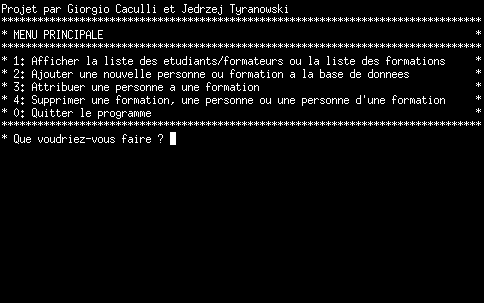
\includegraphics[trim=0 150 0 0, clip, width=\textwidth]{images/01.png}
\end{figure}\\
Pour naviguer dans le menu, il faut frapper entre 0 et 4 sur le clavier et confirmer avec Enter.

\subsubsection{Menu affichage}
\begin{figure}[ht]
  \centering
  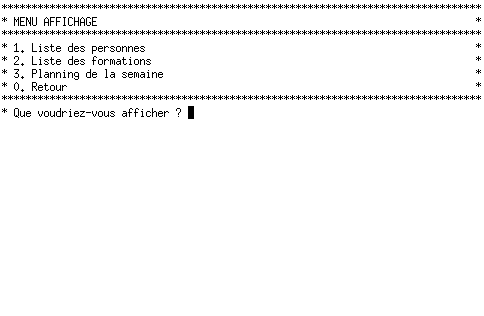
\includegraphics[trim=0 190 0 0, clip, width=\textwidth]{images/02.png}
\end{figure}
Choisissez une option parmi 1, 2 et 3 et confirmez avec Enter pour continuer.

\newpage
\subsubsection{Liste des personnes}
\begin{figure}[ht]
  \centering
  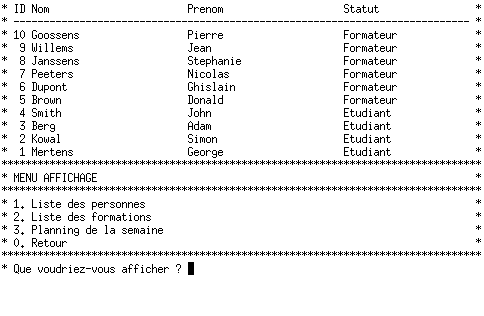
\includegraphics[trim=0 40 0 0, clip, width=\textwidth]{images/03.png}
\end{figure}
Affiche l'ID, le nom de famille, le prénom et le statut (étudiant ou formateur) sous la forme d'une liste.

\subsubsection{Liste des formations}
\begin{figure}[ht]
  \centering
  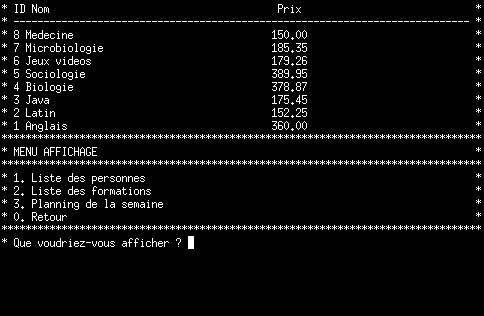
\includegraphics[trim=0 60 0 0, clip, width=\textwidth]{images/04.png}
\end{figure}
Affiche l'ID, le nom et le prix de chaque formation disponible dans la base de données sous la forme d'une liste.

\newpage
\subsubsection{Planning de la semaine}
\begin{figure}[ht]
  \centering
  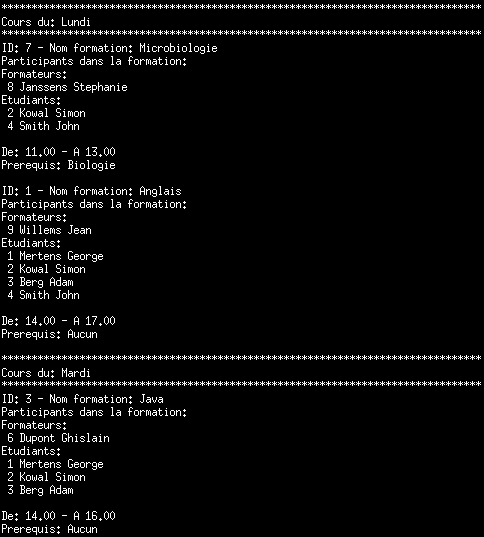
\includegraphics[width=\textwidth]{images/05.png}
\end{figure}
Les informations sont groupées par jour suivi par le nom de la formation, les différents formateurs, les élèves qui y participent et l'horaiare. Les prérequis pour les cours sont dictés en bas, exemple Sociologie est un prérequis pour le cours de Microbiologie

\newpage
\subsubsection{Menu ajout}
\begin{figure}[ht]
  \centering
  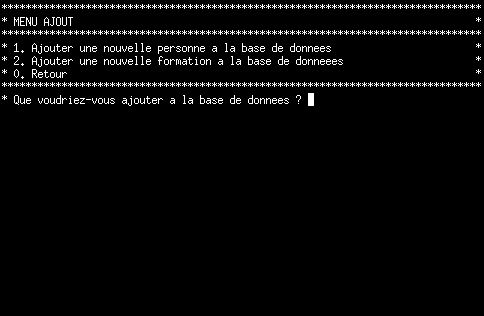
\includegraphics[trim=0 210 0 0, clip, width=\textwidth]{images/06.png}
\end{figure}
Il est possible d'ajouter une nouvelle personne à la base de données ou ajouter une nouvelle formation à la base de données.

\subsubsection{Ajout d'une personne}
\begin{figure}[ht]
  \centering
  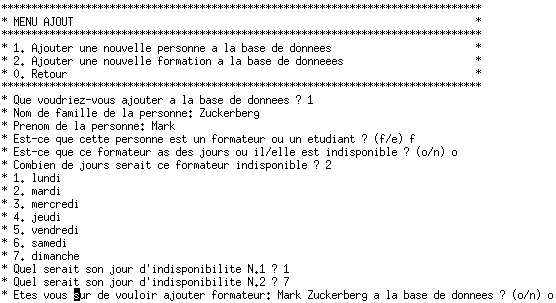
\includegraphics[width=\textwidth]{images/07.png}
\end{figure}
L'ajout d'une personne se passe de la manière suivante:
\begin{enumerate}
\item Il faut insérer son nom de famille.
\item Il faut insérer son prénom.
\item Il faut insérer son statut (étudiant ou formateur), "f" pour formateur, "e" pour étudiant.
\item Il faut insérer le nombre de jours où le formateur est indisponible.
\item Dépendamment du nombre de jour, il faudra attribuer le jour corréspondant à ceux dans la liste ( 1 - lundi, 2 - mardi, etc\ldots)
  \item Il faut confirmer par "o" ou "n" (oui ou non) si l'on souhaite effectivement ajouter la nouvelle personne dans la base de données.
\end{enumerate}

\newpage
\begin{figure}[ht]
  \centering
  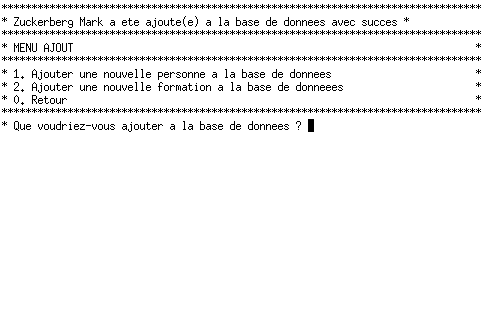
\includegraphics[trim=0 180 0 10, clip, width=\textwidth]{images/08.png}
\end{figure}
Si la personne a été correctement ajoutée à la base de données, un message de confirmation apparaîtra en haut du menu.

\begin{figure}[ht]
  \centering
  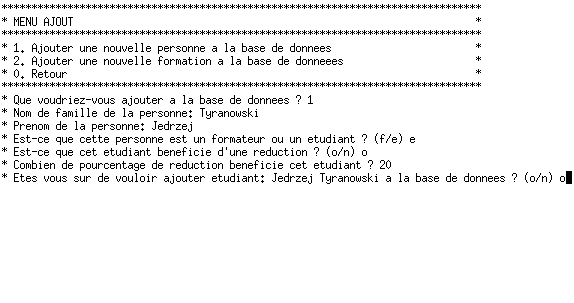
\includegraphics[trim=0 110 0 0, clip, width=\textwidth]{images/09.png}
\end{figure}
Lorsqu'on ajout un étudiant, il faut indiquer son nom de famille, son prénom et la remise éventuelle.

\begin{figure}[ht]
  \centering
  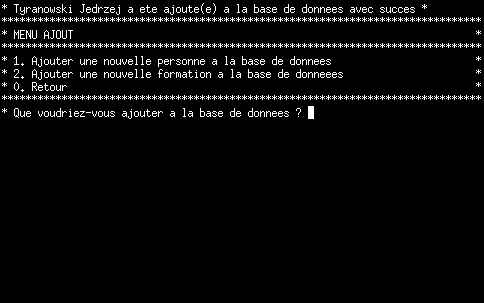
\includegraphics[trim=0 180 0 0, clip, width=\textwidth]{images/10.png}
\end{figure}
Même message de confirmation pour l'étudiant.


\newpage
\subsubsection{Ajout d'une formation}
\begin{figure}[ht]
  \centering
  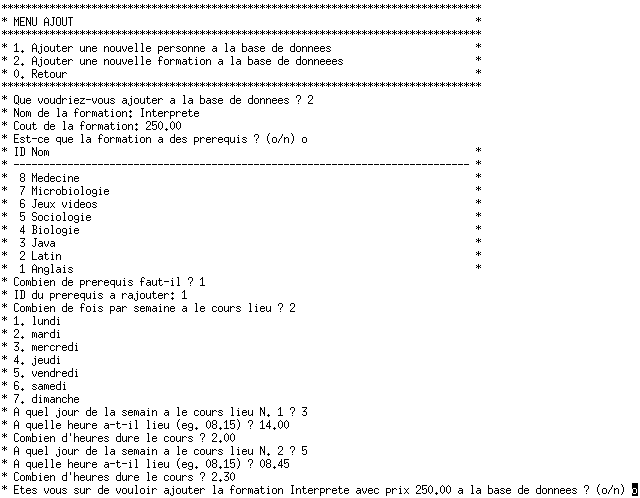
\includegraphics[width=\textwidth]{images/11.png}
\end{figure}
L'ajout d'une formation se passe de la manière suivante:
\begin{enumerate}
\item Il faut insérer son nom.
\item Il faut insérer son prix.
\item Il faut insérer insérer s'il y a des prérequis ou pas par "o" (oui) et "n" (non).
\item Si oui, il faut insérer le nombre de prérequis et l'ID des cours qui seraient des prérequis.
\item Ensuite il faut dire combiends de fois par semaine le cours a lieu.
\item Dépendamment du nombre de jour, il faudra attribuer le jour corréspondant à ceux dans la liste ( 1 - lundi, 2 - mardi, etc\ldots)
\item Il faut insérer vers quelle heure le cours commence. (En format HH.MM)
\item Il faut insérer combien d'heures dure le cours. (En format HH.MM)
\item Il faut confirmer par "o" ou "n" (oui ou non) si l'on souhaite effectivement ajouter la nouvelle personne dans la base de données.
\end{enumerate}

\newpage
\begin{figure}[ht]
  \centering
  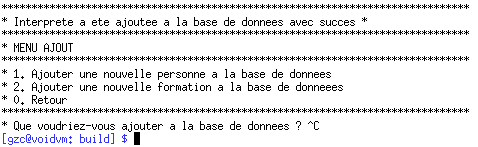
\includegraphics[trim=0 15 10 10, clip, width=\textwidth]{images/12.png}
\end{figure}
Un message de confirmation apparaîtra au dessus du menu.

\newpage
\section{Code}
\subsection{Structures}
Voici les différentes structures qui ont été utilisée dans la conception du programme:

\begin{lstlisting}[firstnumber=30]
  typedef struct personne
  {
    int id;
    char nom[25];
    char prenom[25];
    int formateur;
    int nb_formations;
    int formations[30];
    int nb_jours_indisponible;
    int jours_indisponible[7];
    int reduction;
    int val_reduction;
  } personne;
\end{lstlisting}

Cette structure sert à stocker les informations qui composent une personne quelconque: étudiant ou formateur.\\
Voici ce que représente chaque partie de la structure:
\begin{itemize}
\item \texttt{int id} : L'identifiant unique de la personne.
\item \texttt{char nom[25]} : Le nom de la personne (25 caractères maximum).
\item \texttt{char prenom[25]} : Le prénom de la personne (25 caractères maximum).
\item \texttt{int formateur} : 1 si la personne est un formateur, 0 si la personne est un étudiant.
\item \texttt{int nb\_formations} : Le nombre de formations auquel la personne participera.
\item \texttt{int formations[30]} : Vecteur qui stockera les idéntifiants des différentes formations auquel la personne participera (On suppose dans une année, une personne ne peut participer qu'à 30 formations maximum).
\item \texttt{int nb\_jours\_indisponible} : Si la personne est un formateur, il se peut qu'il/elle ait des jours d'indisponibilé, cette variable va stocker le nombre de jours où cette personne est indisponile (maximum 7).
\item \texttt{int jours\_indisponibles[7]} : Le vecteur qui stockera les jours auquel le formateur ne sera pas disponible(1 - lundi, 2 - mardi, etc\ldots).
\item \texttt{int reduction} : Si la personne est un étudiant, il se peut qu'il ait une réduction sur son minérval, 1 s'il a droit à une réduction, 0 si pas.
\item \texttt{int val\_reduction} : Le pourcentage de réduction auquel un étudiant à droit.
\end{itemize}

\begin{lstlisting}[firstnumber=51]
  typedef struct noeud_db_personne
  {
    personne *p;
    struct noeud_db_personne *next;
  } noeud_db_personne;
\end{lstlisting}

Cette structure sert à devenir les différents n\oe{}uds qui seront stockés dans la base de donnée, soit la structure \texttt{db\_personne}.
Voici ce qui représent chaque partie de la structure:
\begin{itemize}
\item \texttt{personne *p} : Le pointeur de la personne qui sera stocké dans ce n\oe{}ud lors de sa création.
\item \texttt{struct noeud\_db\_personne *next} : qui contiendra le tête lors qu'on créera un nouveau n\oe{}ud, sinon \texttt{NULL}.
\end{itemize}

\begin{lstlisting}[firstnumber=63]
  typedef struct db_personne
  {
    noeud_db_personne *head;
  } db_personne;
\end{lstlisting}

Cette structure sert à contenir tous les différentes n\oe{}uds \texttt{noeud\_db\_personne}. C'est à partir de cette structure que l'on stockera les différentes n\oe{}uds qui eux-mêmes stockeront leurs personnes respectives.
\begin{itemize}
\item \texttt{noeud\_db\_personne *head} : La tête de la liste chaînée qui stockera toutes les personnes.
\end{itemize}

\begin{lstlisting}[firstnumber=73]
  typedef struct noeud_formation
  {
    personne *p;
    struct noeud_formation *next;
  } noeud_formation;
\end{lstlisting}

Cette structure va stocker les différentes personnes qui participeront à une formation spécifique.
\begin{itemize}
\item \texttt{personne *p} : La personne qui participera à la formation.
\item \texttt{struct noeud\_formation *next} : Le n\oe{}ud de pour la prochaine personne qui sera stockée.
\end{itemize}

\begin{lstlisting}[firstnumber=94]
  typedef struct formation
  {
    int id;
    char nom[40];
    float prix;
    int nb_jours;
    int jours[7];
    float heures[24];
    float durees[10];
    int nb_prerequis;
    int prerequis[10];
    noeud_formation *head;
  } formation;
\end{lstlisting}

Cette structure sert à stocker toutes les informations qui composent une formations.
Voici ce que chaque partie représente:
\begin{itemize}
\item \texttt{int id} : L'identifiant unique de la formation.
\item \texttt{char nom[40]} : Le nom de la formation (40 caractères maximum).
\item \texttt{float prix} : Le coût de la formation.
\item \texttt{int nb\_jours} : Le nombre de jours par semaine où cette formation à cours.
\item \texttt{int jours[7]} : Vecteur contenant les jours où la formation a cours.
\item \texttt{float heures[24]} : Le nombre d'heures du début de la formation.
\item \texttt{float durees[10]} : Les différentes durées du cours lors de la semaine.
\item \texttt{int nb\_prerequis} : Le nombre de prérequis pour avoir accès à cette formation.
\item \texttt{int prerequis[10]} : Vecteur contenant les identifiants des formations qui seraient des prérequis.
\item \texttt{noeud\_formation *head} : Étant donné qu'une formation stocke des personnes, elle-même est une liste chaînée qui stockera un nombre indéterminé de participants.
\end{itemize}

\begin{lstlisting}[firstnumber=115]
  typedef struct noeud_db_formation
  {
    formation *f;
    struct noeud_db_formation *next;
  } noeud_db_formation;
\end{lstlisting}

Cette structure suit la même logique que la structure \texttt{noeud\_db\_personne}. Elle sert à stocker les différentes formations, qui eux-mêmes stockeront les personnes à leurs tour.
\begin{itemize}
\item \texttt{formation *f} : La formation qui sera stockée dans la base de données.
\item \texttt{struct noeud\_db\_formation *next} : La prochaine formation qui sera stockée dans la base de données. \texttt{NULL} si pas de prochaine formation.
\end{itemize}

\begin{lstlisting}[firstnumber=127]
  typedef struct db_formation
  {
    noeud_db_formation *head;
  } db_formation;
\end{lstlisting}

Cette structure aussi suit la même logique que la structure \texttt{db\_formation}. Elle sert de tête pour la la liste chaînée et c'est à partir de cette structure-ci que l'on démarrera les différentes interactions avec la base de données des formations.
\begin{itemize}
\item \texttt{noeud\_db\_formation *head} : La tête de la liste chaînée qui stockera les différentes formations.
\end{itemize}

Pourquoi avons-nous choisi cette approche ? Principalement car on ne voulait pas stocker les différentes personnes et les différentes formations dans des vecteurs. On ne voulait pas qu'il y ait un nombre prédéfini de personnes et un nombre prédéfini de formations, on s'est donc fiés aux listes chaînées. Et c'est pourquoi maintenant il est possible de stocker autant de formations que la \acrshort{ram} nous permet ainsi que de stocker autant de formations que la \acrshort{ram} nous permet.

\newpage
\subsection{Fonctions}
\subsubsection{Fonctions qui créent des n\oe{}ds}
Voici les différentes fonctions que l'on a du créer pour le bon fonctionnement du programme:
\begin{lstlisting}[firstnumber=144]
  personne *creer_personne( char nom[], char prenom[], int formateur );
\end{lstlisting}

Cette fonction sert à créer un pointeur qui permettra d'initialiser les différentes informations présentes dans la structure \texttt{personne}. Lors de l'initialisation d'une personne, on n'aura besoin que du nom de famille de la personne, son prenom et s'il/elle est un formateur ou pas. Le reste des informations est manipulé par la suite lors des différentes interactions.

\begin{lstlisting}[firstnumber=168]
  db_personne *creer_db_personne();
\end{lstlisting}

Cette fonction sert à initialiser le pointer \texttt{noeud\_db\_personne *head} dans la structure \texttt{db\_personne} à \texttt{NULL}, afin que l'on puisse commencer à faire des manipulations avec cette structure.

\begin{lstlisting}[firstnumber=303]
  formation *creer_formation( char nom[], float prix );
\end{lstlisting}

Cette fonction sert à créer un pointeur qui permettra d'initialiser les différentes informations présentes dans la structure \texttt{formation}. Lors de l'initialisation d'une formation, on n'aura besoin que du nom de la formation et de son prix. Le reste des informations est manipulé par la suite lors des différentes interactions.

\begin{lstlisting}[firstnumber=442]
  db_formation *creer_db_formation();
\end{lstlisting}

Cette fonction sert à initialiser le pointer \texttt{noeud\_db\_formation *head} dans la structure \texttt{db\_formation} à \texttt{NULL}, afin que l'on puisse commencer à faire des manipulations avec cette structure.

\subsubsection{Fonctions qui affichent des listes chaînées}

\begin{lstlisting}[firstnumber=157]
  void afficher_personne( personne *p );
\end{lstlisting}

Cette fonction sert à afficher les informations de base qui caractérisent une \textbf{personne}. De manière générale, son identifiant, son nom de famille, son prénom et s'il est formateur ou étudiant.

\begin{lstlisting}[firstnumber=257]
  void afficher_db_personne( db_personne *db );
\end{lstlisting}

Cette fonction parcourt l'entièreté de la base de données \texttt{db\_personne *db}. Tant que la tête n'est pas \texttt{NULL}, on affichera les informations que l'on souhaite afficher de chaque personne présente dans la base de données.

\begin{lstlisting}[firstnumber=408]
  void afficher_formation( formation *f );
\end{lstlisting}

Cette fonction sert à afficher les informations de base qui caractérisent une \textbf{formation}. De manière générale, son identifiant, son nom, son prix, ainsi que les personnes qui y participent.

\begin{lstlisting}[firstnumber=461]
  void afficher_db_formation( db_formation *dbf );
\end{lstlisting}

Cette fonction parcourt l'entièreté de la base de données \texttt{db\_formation *dbf}. Tant que la tête n'est pas \texttt{NULL}, on affichera les informations que l'on souhaite afficher de chaque formation présente dans la base de données.

\subsubsection{Fonctions qui ajoutent un n\oe{}ud à une liste chaînée}

\begin{lstlisting}[firstnumber=187]
  void ajouter_db_personne( db_personne *db, personne *p );
\end{lstlisting}

Cette fonction sert à initialiser un pointeur \texttt{noeud\_db\_personne *ndb} qui stockera \texttt{personne *p} dans la base de données \texttt{db\_personne *db}. Ici, l'ajout dans la liste chaînée à lieu par le mécanisme suivant:
\begin{enumerate}
\item On initialise le noeud temporaire que l'on ajoutera à la base de données.
\item On associe \texttt{p} au pointeur \texttt{p} présent dans la structure \texttt{noeud\_db\_personne}.
\item On initialise le prochain n\oe{}ud de la liste \texttt{*next} à NULL.
\item Si la tête \texttt{*head} de la base de donnée est \texttt{NULL}, alors la tête devient le nouveau n\oe{}ud. On arrête la fonction d'ajout là.
\item Sinon, on fait une copie de la tête dans le n\oe{}ud \texttt{*next} que l'on avait initialisé à \texttt{NULL}.
\item On déclare la tête comme étant le n\oe{}ud temporaire que l'on a initialisé.
\end{enumerate}

\begin{lstlisting}[firstnumber=322]
  int ajouter_formation( formation *f, personne *p );
\end{lstlisting}

Cette fonction sert à initialiser un pointeur \texttt{noeud\_formation *nf} qui stockera \texttt{personne *p} qui participera dans \texttt{formation *f}. Ici, l'ajout dans la liste chaînée à lieu par le mécanisme suivant:
\begin{enumerate}
\item On initialise le noeud temporaire que l'on ajoutera dans la formation.
\item On associe \texttt{p} au pointeur \texttt{p} présent dans la structure \texttt{noeud\_formation}.
\item On initialise le prochain n\oe{}ud de la liste \texttt{*next} à NULL.
\item Si la tête \texttt{*head} de la formation est \texttt{NULL}, alors la tête devient le nouveau n\oe{}ud. On arrête la fonction d'ajout là.
\item Sinon, on fait une copie de la tête dans le n\oe{}ud \texttt{*next} que l'on avait initialisé à \texttt{NULL}.
\item On déclare la tête comme étant le n\oe{}ud temporaire que l'on a initialisé.
\end{enumerate}

\begin{lstlisting}[firstnumber=559]
  void ajouter_db_formation( db_formation *db, formation *f );
\end{lstlisting}

Cette fonction sert à initialiser un pointeur \texttt{noeud\_db\_formation *ndb} qui stockera \texttt{formation *f} dans la base de données \texttt{db\_formation *db}. Ici, l'ajout dans la liste chaînée à lieu par le mécanisme suivant:
\begin{enumerate}
\item On initialise le noeud temporaire que l'on ajoutera à la base de données.
\item On associe \texttt{f} au pointeur \texttt{f} présent dans la structure \texttt{noeud\_db\_formation}.
\item On initialise le prochain n\oe{}ud de la liste \texttt{*next} à NULL.
\item Si la tête \texttt{*head} de la base de donnée est \texttt{NULL}, alors la tête devient le nouveau n\oe{}ud. On arrête la fonction d'ajout là.
\item Sinon, on fait une copie de la tête dans le n\oe{}ud \texttt{*next} que l'on avait initialisé à \texttt{NULL}.
\item On déclare la tête comme étant le n\oe{}ud temporaire que l'on a initialisé.
\end{enumerate}

\subsubsection{Fonctions qui suppriment un n\oe{}ud d'une liste chaînée}

\begin{lstlisting}[firstnumber=216]
  int supprimer_db_personne( db_personne *dbp, int id );
\end{lstlisting}

Cette fonction sert à supprimer une personne de la base de données à partir de son identifiant. La démarche faite dans cette fonction est la suivant:
\begin{enumerate}
\item On vérife que la tête de la base de données \texttt{dbp->head} ne soit pas \texttt{NULL}, si oui, on arrête la fonction.
\item On vérifie si le premier élément de la liste correspond à l'\texttt{id} de la personne que l'on souhaite supprimer.
\item Si oui:
  \begin{enumerate}
  \item On crée un n\oe{}ud temporaire qui stockera la personne suivante dans la liste.
  \item On libére l'espace mémoire occupé par head avec la fonction \texttt{free(dbp->head)}.
  \item On attribue à \texttt{dbp->head} le n\oe{}ud temporaire que l'on avait créé.
  \item On arrête la fonction.
  \end{enumerate}
\item Sinon, on parcourt l'entièreté de la liste jusqu'au moment où l'on trouve la personne qui a le même \texttt{id} que l'\texttt{id} en paramètre.
\item Si on le trouve, on pivote l'élément qui suit vers l'élément que l'on vient de supprimer.
\item On arrête la fonction, si réussite, on obtient 1, si pas, on obtient 0.
\end{enumerate}

\begin{lstlisting}[firstnumber=361]
  int supprimer_personne_de_formation( formation *f, int id );
\end{lstlisting}

Cette fonction sert à supprimer une personne de la fonction à partir de son identifiant. La démarche faite dans cette fonction est la suivant:
\begin{enumerate}
\item On vérife que la tête de la fonction \texttt{f->head} ne soit pas \texttt{NULL}, si oui, on arrête la fonction.
\item On vérifie si le premier élément de la liste correspond à l'\texttt{id} de la personne que l'on souhaite supprimer.
\item Si oui:
  \begin{enumerate}
  \item On crée un n\oe{}ud temporaire qui stockera la personne suivante dans la liste.
  \item On libére l'espace mémoire occupé par head avec la fonction \texttt{free(f->head)}.
  \item On attribue à \texttt{f->head} le n\oe{}ud temporaire que l'on avait créé.
  \item On arrête la fonction.
  \end{enumerate}
\item Sinon, on parcourt l'entièreté de la liste jusqu'au moment où l'on trouve la personne qui a le même \texttt{id} que l'\texttt{id} en paramètre.
\item Si on le trouve, on pivote l'élément qui suit vers l'élément que l'on vient de supprimer.
\item On arrête la fonction, si réussite, on obtient 1, si pas, on obtient 0.
\end{enumerate}

\begin{lstlisting}[firstnumber=490]
  int supprimer_db_formation( db_formation *dbf, int id );
\end{lstlisting}

Cette fonction sert à supprimer une formation de la base de données à partir de son identifiant. La démarche faite dans cette fonction est la suivant:
\begin{enumerate}
\item On vérife que la tête de la base de données \texttt{dbf->head} ne soit pas \texttt{NULL}, si oui, on arrête la fonction.
\item On vérifie si le premier élément de la liste correspond à l'\texttt{id} de la formation que l'on souhaite supprimer.
\item Si oui:
  \begin{enumerate}
  \item On crée un n\oe{}ud temporaire qui stockera la formation suivante dans la liste.
  \item On libére l'espace mémoire occupé par head avec la fonction \texttt{free(dbf->head)}.
  \item On attribue à \texttt{dbf->head} le n\oe{}ud temporaire que l'on avait créé.
  \item On arrête la fonction.
  \end{enumerate}
\item Sinon, on parcourt l'entièreté de la liste jusqu'au moment où l'on trouve la formation qui a le même \texttt{id} que l'\texttt{id} en paramètre.
\item Si on le trouve, on pivote l'élément qui suit vers l'élément que l'on vient de supprimer.
\item On arrête la fonction, si réussite, on obtient 1, si pas, on obtient 0.
\end{enumerate}

\subsubsection{Fonctions qui servent de \texttt{getter()}}

\begin{lstlisting}[firstnumber=275]
  personne *get_personne( db_personne *db, char nom[], char prenom[], int formateur );
\end{lstlisting}

Cette fonction renvoie \texttt{NULL} si une personne d'un nom spécifique, d'un prénom spécifique, et s'il est formateur ou étudiant n'existe pas dans la base de données \texttt{db\_personne *db}. Sinon, la fonction retourne la personne trouvée.

\begin{lstlisting}[firstnumber=532]
  formation *get_formation( db_formation *dbf, char nom_formation[] );
\end{lstlisting}

Cette fonction renvoie \texttt{NULL} si une formation avec un nom spécifique n'existe pas dans la base de données \texttt{db\_formation *dbf}. Sinon, la fonction retourne la formation trouvée.

\subsubsection{Fonctions qui affiches les différentes parties du menu interactif}
les fonctions ci-dessous ne servent qu'à affichier les différentes parties du menu interactif. Elle ne font aucune manipulation particulière autre qu'affichier du texte.
\begin{lstlisting}
  void menu_creer_formation( db_formation *f );
\end{lstlisting}

\begin{lstlisting}
  void menu_creer_personne( db_personne *p );
\end{lstlisting}

\begin{lstlisting}
  int menu_creer( db_formation *f, db_personne *p );
\end{lstlisting}

\begin{lstlisting}
  void menu_ajouter_formation( db_formation *f, db_personne *p );
\end{lstlisting}

\begin{lstlisting}
  void menu_supprimer_personne( db_formation *dbf, db_personne *dbp );
\end{lstlisting}

\begin{lstlisting}
  void menu_supprimer_formation( db_formation *dbf, db_personne *dbp );
\end{lstlisting}

\begin{lstlisting}
  int menu_supprimer_personne_de_formation( db_formation *dbf );
\end{lstlisting}

\begin{lstlisting}
  int menu_supprimer( db_formation *dbf, db_personne *dbp );
\end{lstlisting}

\begin{lstlisting}
  int menu_affichage( db_formation *f, db_personne *p );
\end{lstlisting}

\begin{lstlisting}
  int menu( db_formation *f, db_personne *p );
\end{lstlisting}

\begin{lstlisting}
  int main( void );
\end{lstlisting}

\newpage
\printglossary

\end{document}
